\subsection{Processo di sviluppo}
\label{subsection:processo_sviluppo}
ll processo di sviluppo riguarda l'insieme di attività necessarie per produrre e implementare il software, assicurandosi che risponda ai requisiti definiti e sia di qualità adeguata.

\subsubsection{Analisi dei requisiti}
L'analisi dei requisiti è una attività cruciale nel ciclo di vita del software, in cui vengono raccolte, analizzate e documentate le esigenze degli stakeholder per definire chiaramente cosa il sistema dovrà fare. 
Questa attività produce il documento di analisi dei requisiti descritto nella sezione \hyperref[subsec:documentazione]{Documentazione}.

\paragraph{Requisiti}
I requisiti vengono categorizzati in:
\begin{enumerate}
    \item \textbf{Requisiti funzionali}.
    
    Rappresentano ciò che un sistema deve fare per soddisfare le esigenze degli utenti o degli stakeholders.

    \item \textbf{Requisiti qualitativi}.
    
    I requisiti di qualità (requisiti non funzionali) descrivono caratteristiche qualitative del sistema, come prestazioni, sicurezza, usabilità e manutenibilità.

    \item \textbf{Di vincolo}.
    
    I requisiti di vincolo rappresentano limitazioni o condizioni obbligatorie che influenzano lo sviluppo, l'implementazione o l'operatività del sistema. 
    A differenza dei requisiti funzionali o di qualità, non descrivono cosa deve fare il sistema, ma come deve essere realizzato rispettando regole o restrizioni specifiche. 

    \item \textbf{Prestazionali}.
    
    I requisiti prestazionali sono un tipo specifico di requisiti non funzionali che definiscono le aspettative relative alle prestazioni del sistema.
    Alcuni esempi sono: la velocità, il tempo di risposta, la capacità di carico, e altre caratteristiche misurabili legate all'efficienza.
\end{enumerate}


\paragraph{Casi d'uso}
\label{par:casi_uso}
I casi d'uso forniscono una descrizione dettagliata delle funzionalità del sistema dal punto di vista degli utenti, delineando come il sistema risponda a specifiche azioni o scenari. 
In particolare un caso d'uso rappresenta un uso completo del sistema dalla prospettiva dell'utente.
I casi d'uso vengono rappresentati tramite una combinazione di descrizione e diagramma UML.
Durante la definizione di un caso d'uso possono emergere nuove informazioni che richiedono una modifica dei casi d'uso definiti in precedenza.
La definizione dei casi d'uso non è quindi lineare.

\subparagraph{Descrizione}
Nella \hyperref[tab:template_casi_uso]{Tabella \ref{tab:template_casi_uso}} viene mostrato il template per la descrizione dei casi d'uso.
Ogni descrizione di caso d'uso deve includere:
\begin{enumerate}
    \item \textbf{Identificativo}.
    
    \texttt{UC-<ID caso principale>.<ID sotto caso>}. 
    
    Dove:
    \begin{enumerate}
        \item \texttt{<ID caso principale>}: identificativo numerico del caso d'uso principale (numero crescente).

        \item \texttt{<ID sotto caso>}: identificativo numerico del sotto caso d'uso (presente solo se si tratta di un sotto caso d'uso).
    \end{enumerate}

    \item \textbf{Requisito utente}.
    
    Requisito utente a cui fa riferimento il diagramma.

    \item \textbf{Pre-condizioni}.
    
    Stato iniziale del sistema o vincoli necessari per l'attivazione del caso d'uso.

    \item \textbf{Post-condizioni}.
    
    Stato finale del sistema dopo un esecuzione normale(priva di errori) del caso d'uso.

    \item \textbf{Attori}.
    Un attore è un entità esterna(\underline{umana o meno}) al sistema che interagisce con il sistema per iniziare o per contribuire al compimento dell'esecuzione di un caso d'uso.  
    Gli attori si dividono in:
    \begin{enumerate}
        \item  \textbf{Attori primari}: attori principali che partecipano al caso d'uso, solitamente contengono gli attori che iniziano l'interazione e/o sono i destinatari delle informazioni in output del caso d'uso.
        \item \textbf{Attore secondario}: altri attori coinvolti che non sono protagonisti nell'esecuzione del caso d'uso(es. Sistemi esterni).
    \end{enumerate}

    \item \textbf{Trigger}.
    
    Evento eseguito da un attore che attiva il caso d'uso.

    \item \textbf{Scenario principale}.
    
    La sequenza di step importanti che vengono portati a termine in un esecuzione normale del caso d'uso.
    
    \item \textbf{Scenari alternativi}.

    Eventuali deviazioni o eccezioni rispetto allo scenario principale.
\end{enumerate}

\begin{usecase}{\texttt{<identificativo caso d'uso>}}{\texttt{<descrizione caso d'uso>}}
            
    \req{\texttt{<link requisito utente>}}
    
    \pre{
        \item \texttt{<pre condizione>}
        \item \texttt{<pre condizione>}
    }
    
    \post {
        \item \texttt{<post condizione>}
        \item \texttt{<post condizione>}
    }
    
    \actor{\texttt{<attore principale>}}
    
    \subactors{\texttt{<lista attori secondari>}}

    \trigger{\texttt{<trigger>}}
    
    \inc{\texttt{<lista casi d'uso inclusi>}}
    
    \base{\texttt{<caso d'uso di base>}}
    
    \scenario{
        \item \texttt{<$1^a$ azione>}
        \item \texttt{<$2^a$ azione>}
        \item \texttt{<<include:id>>}
    }

    \subscenario{
        \item[1.1] \texttt{<condizione branch dalla $1^a$ azione>}
        \begin{itemize}
            \item [a.] \texttt{$1^a$ azione del scenario secondario}
            \item [b.] \texttt{$2^a$ azione del scenario secondario}
        \end{itemize} 
        \item[2.1] \texttt{<condizione branch dalla $2^a$ azione>}
        \begin{itemize}
            \item [a.] \texttt{$1^a$ azione del scenario secondario}
            \item [b.] \texttt{$2^a$ azione del scenario secondario}
        \end{itemize} 
    }
    \caption{Template casi d'uso.}
    \label{tab:template_casi_uso}
\end{usecase}


\subparagraph{Diagrammi dei casi d'uso}
I diagrammi dei casi d'uso sono strumenti grafici utilizzati nell'ingegneria del software per rappresentare in modo intuitivo le interazioni tra gli utenti (attori) e un sistema. Basati sul linguaggio UML (Unified Modeling Language), questi diagrammi illustrano i principali scenari operativi del sistema e aiutano a identificare e chiarire i requisiti funzionali.
Ogni diagramma è composto da:
\begin{itemize}
    \item \textbf{Sistema}: delimita i confini del sistema software, indicando quali funzionalità sono incluse e quali sono esterne a esso.
    Il sistema viene rappresentato nei diagrammi come mostrato in \hyperref[fig:sistema_uml]{Figura \ref{fig:sistema_uml}}.
    \begin{figure}[H]
        \centering
        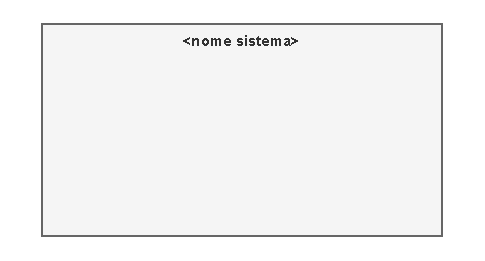
\includegraphics{Sezioni/ProcessiPrimari/Immagini/sistema_caso_uso.pdf}
        \caption{Rappresentazione del sistema in UML.}
        \label{fig:sistema_uml}
    \end{figure}
    
    \item \textbf{Attori}: rappresentano soggetti che interagiscono con il sistema software. Gli attori possono essere persone, altri applicativi o dispositivi che utilizzano le funzionalità del sistema.
    Un attore viene rappresentato nei diagrammi usando una delle due notazioni mostrate in \hyperref[fig:attori_uml]{Figura \ref{fig:attori_uml}} posta al di fuori del sistema.
    \begin{figure}[H]
        \centering
        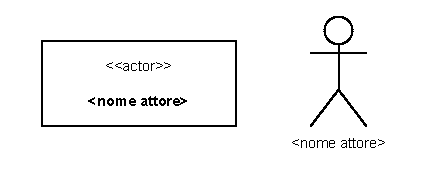
\includegraphics{Sezioni/ProcessiPrimari/Immagini/attori_caso_uso.pdf}
        \caption{Rappresentazione degli attori in UML.}
        \label{fig:attori_uml}
    \end{figure}
    
    \item \textbf{Casi d'uso}: rappresentano le funzionalità o i servizi offerti dal sistema che producono un risultato di valore per un attore. Ogni caso d'uso descrive una sequenza specifica di interazioni tra gli attori e il sistema.
    Ogni caso d'uso viene rappresentato nei diagrammi usando la notazione mostrata in \hyperref[fig:caso_uso]{Figura \ref{fig:caso_uso}} posta all'interno del sistema.
    \begin{figure}[H]
        \centering
        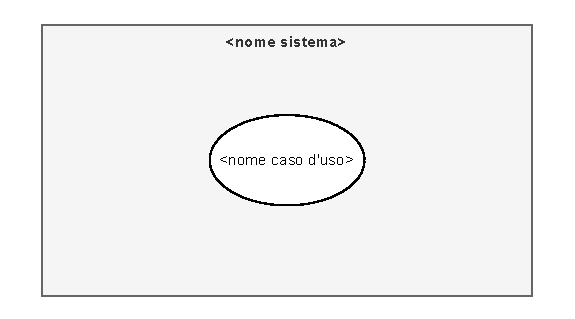
\includegraphics{Sezioni/ProcessiPrimari/Immagini/caso_uso.pdf}
        \caption{Rappresentazione caso d'uso in UML.}
        \label{fig:caso_uso}
    \end{figure}
    
    \item \textbf{Relazioni}.
    
    Sono delle notazioni che permettono di rendere più modulari i diagrammi di casi d'uso e di rendere chiara l'interazione degli attori con il sistema.
    
    \begin{itemize}
        \item \textbf{Associazione}: è la relazione fondamentale che collega un attore a un caso d'uso a cui esso partecipa.
        Uno stesso attore può partecipare a \texttt{N} casi d'uso.
        Le associazioni vengono rappresentate in UML come mostrato in \hyperref[fig:associazione_uml]{Figura \ref{fig:associazione_uml}}.
        \begin{figure}[H]
            \centering
            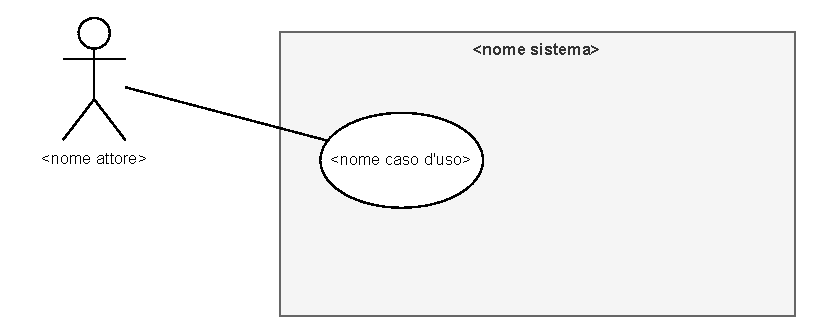
\includegraphics{Sezioni/ProcessiPrimari/Immagini/associazione_uml.pdf}
            \caption{Rappresentazione associazione in UML.}
            \label{fig:associazione_uml}
        \end{figure}

        \item \textbf{Inclusione}: rappresenta una dipendenza in cui il comportamento del caso d'uso incluso è incorporato ogni volta che viene eseguito il caso d'uso base. Il caso d'uso incluso contiene funzionalità che sono riutilizzate in più casi d'uso principali, permettendo di evitare la duplicazione di comportamenti comuni.
        L'inclusione viene rappresentata in UML come mostrato in \hyperref[fig:inclusione_uml]{Figura \ref{fig:inclusione_uml}}.
        \begin{figure}[H]
            \centering
            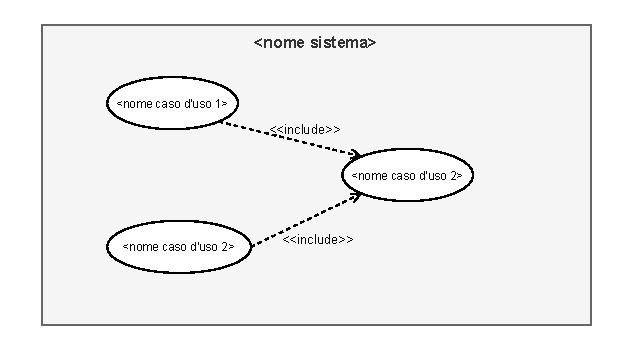
\includegraphics{Sezioni/ProcessiPrimari/Immagini/inclusione_uml.pdf}
            \caption{Rappresentazione inclusione in UML.}
            \label{fig:inclusione_uml}
        \end{figure}
        Come si può vedere nella \hyperref[tab:template_casi_uso]{Tabella \ref{tab:template_casi_uso}} è necessario:
        \begin{enumerate}
            \item Indicare il caso d'uso incluso come valore della colonna "Casi d'uso inclusi".
            \item Indicare lo step dello scenario principale o delle estensioni che utilizza il caso d'uso incluso.
            Questo viene fatto tramite la sintassi \texttt{include::<nome caso d'uso>}.
        \end{enumerate} 

        \item \textbf{Estensione}: mostra una relazione in cui un caso d'uso esteso aumenta le funzionalità del caso d'uso principale. Il caso d'uso esteso viene eseguito solo sotto determinate condizioni, interrompendo l'esecuzione del caso d'uso principale.
        L'estensione viene rappresentata in UML come mostrato in \hyperref[fig:estensione_uml]{Figura \ref{fig:estensione_uml}}.
        \begin{figure}[H]
            \centering
            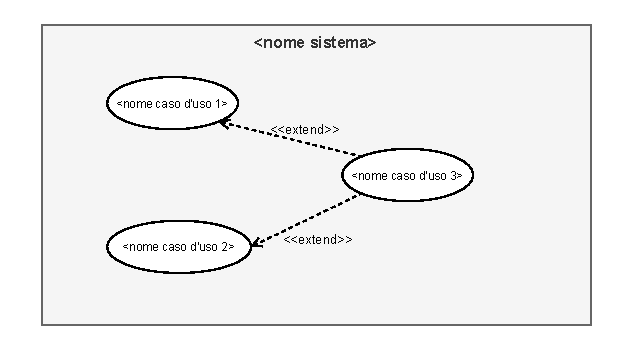
\includegraphics{Sezioni/ProcessiPrimari/Immagini/estensione_uml.pdf}
            \caption{Rappresentazione estensione in UML.}
            \label{fig:estensione_uml}
        \end{figure}
        
        \item \textbf{Generalizzazione}: rappresenta una relazione in cui un caso d'uso figlio può aggiungere funzionalità o modificare il comportamento di un caso d'uso genitore. Tutte le funzionalità definite nel caso d'uso genitore si mantengono nel caso d'uso figlio se queste non vengono ridefinite.
        La generalizzazione viene rappresentata in UML come mostrato in \hyperref[fig:generalizzazione_uml]{Figura \ref{fig:generalizzazione_uml}}.
        \begin{figure}[H]
            \centering
            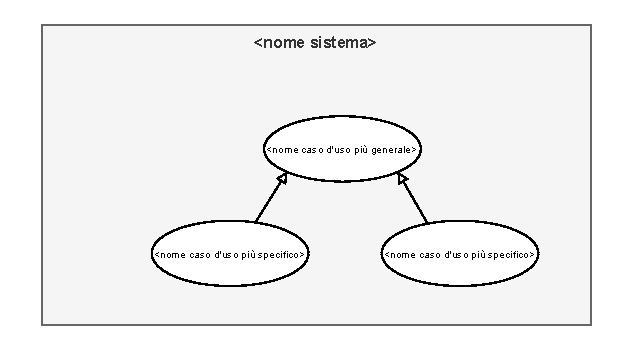
\includegraphics{Sezioni/ProcessiPrimari/Immagini/generalizzazione_uml.pdf}
            \caption{Rappresentazione generalizzazione in UML.}
            \label{fig:generalizzazione_uml}
        \end{figure}
        Come si può vedere nella \hyperref[tab:template_casi_uso]{Tabella \ref{tab:template_casi_uso}} è necessario indicare il caso d'uso genitore come valore della colonna "Caso d'uso base".

    \end{itemize}

    \item \textbf{Sottocasi d'uso}: i sottocasi d'uso rappresentano scenari specifici e dettagliati che si sviluppano all'interno di un caso d'uso principale. La loro funzione è di descrivere in modo approfondito le diverse situazioni o varianti operative che possono verificarsi nel contesto del caso d'uso generale.
    In particolare, ogni caso d'uso può essere suddiviso in più sottocasi, ciascuno associato a una specifica pagina o componente funzionale correlata al caso d'uso principale.
    
\end{itemize}

\paragraph{Fonti per l'Individuazione dei Casi d'Uso}
L'individuazione dei casi d'uso si basa principalmente sul capitolato fornito, che rappresenta una fonte essenziale per comprendere le caratteristiche generali del software da realizzare. 
Il capitolato, descrive le funzionalità principali e gli obiettivi del sistema, specificando alcuni requisiti chiave. 

Tuttavia, non tutti gli aspetti operativi sono dettagliati nel documento, il che rende necessaria un'integrazione attraverso deduzioni basate su necessità logiche e conoscenze pregresse. 
Il capitolato guida l'identificazione delle macro interazioni, consentendo di delineare i casi d'uso principali e il contesto generale in cui il sistema opererà. 
Tuttavia, nei punti in cui le specifiche risultano incomplete o generiche, è indispensabile adottare un approccio pro attivo, immaginando scenari d'uso che derivano dall'analisi delle esigenze tipiche di sistemi simili e delle best practices nel settore.

Questa attività di interpretazione si traduce nella definizione di ulteriori dettagli operativi, come eccezioni o varianti necessarie per garantire una piena copertura dei processi e un corretto funzionamento del sistema.

\subparagraph{Individuazione dei casi d'uso}
L'identificazione dei casi d'uso avviene attraverso i seguenti passaggi:
\begin{enumerate}
    \item \textbf{Identificazione degli attori}: Gli attori sono individuati in base ai loro ruoli e alle loro necessità operative. 
    Ad esempio, in un sistema gestionale possono essere individuati attori come l'amministratore, l'utente finale e un sistema di terze parti che si integra per la gestione dei pagamenti.
    L'identificazione degli attori è fondamentale per comprendere chi interagirà con il sistema e quali sono le operazioni che gli utenti devono poter eseguire.
    In \hyperref[fig:identificare_attori]{Figura \ref{fig:identificare_attori}} viene mostrata una tecnica utile per decidere se un concetto che appare nei requisiti è un attore o meno.
    \begin{figure}[H]
        \centering
        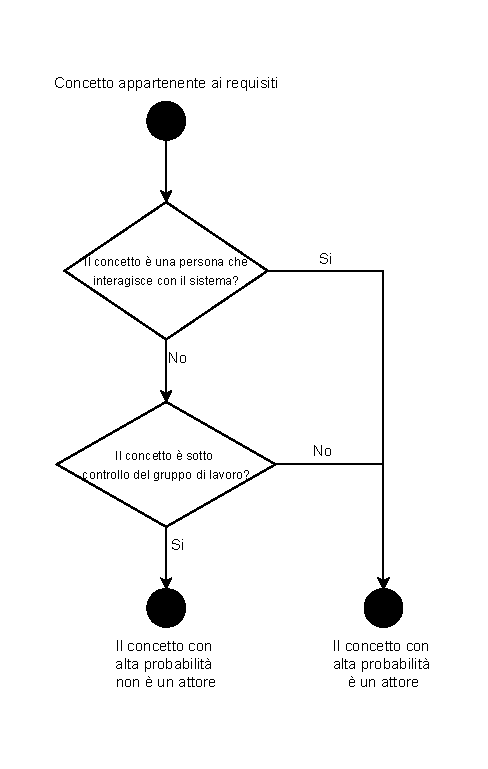
\includegraphics{Sezioni/ProcessiPrimari/Immagini/tecnica_casi_uso.pdf}
        \caption{Tecnica per identificare gli attori.}
        \label{fig:identificare_attori}
    \end{figure} 

    \item \textbf{Raffinamento attori}: Una coppia di attori può essere in una particolare relazione chiamata generalizzazione.
    In questa relazione l'attore "più generale" può eseguire un insieme di interazioni con il sistema che sono un sotto insieme delle interazioni che può eseguire l'attore "più specializzato".
    In altre parole l'attore "più specializzato" può eseguire tutte le interazioni che può eseguire l'attore "più generico" più eventuali ulteriori interazioni.
    In questo passaggio è importante scoprire queste relazioni tra gli attori.

    \item \textbf{Analisi degli obiettivi degli attori}: Una volta identificati gli attori e le relazioni tra essi, vengono analizzati i loro obiettivi in relazione al sistema. 
    Questo processo si basa sulla comprensione dei risultati che ogni attore desidera ottenere, come ad esempio la gestione di un ordine, l'accesso a report personalizzati o la possibilità di modificare parametri di configurazione.
    Gli obiettivi degli attori aiutano a delineare il perimetro dei casi d'uso e a definire le funzionalità che il sistema deve supportare per soddisfare tali obiettivi.

    \item \textbf{Identificazione dei casi d'uso principali}: Partendo dagli obiettivi individuati, si procede con la definizione dei casi d'uso principali. Questi rappresentano le macro funzionalità del sistema, cioè le interazioni essenziali e più frequenti tra gli attori e il sistema stesso. Ogni caso d'uso principale viene descritto in termini di azioni, e risultati attesi, garantendo che le funzionalità fondamentali siano chiaramente delineate.
    
    \item \textbf{Scomposizione in sotto-casi}: I casi d'uso principali possono venire successivamente scomposti in sotto-casi, se necessario, per dettagliare specifiche eccezioni, varianti o processi secondari. Questa scomposizione permette di descrivere scenari più specifici o complessi che possono verificarsi durante l'interazione. Ad esempio, il caso d'uso principale "Gestione di un ordine" può essere suddiviso nei sotto-casi "Modifica di un ordine esistente" e "Cancellazione di un ordine in attesa". Questo livello di dettaglio consente di rappresentare in modo accurato e completo tutti i comportamenti attesi del sistema.

\end{enumerate}